% ___________________________________________
    % Questionnaire respondents
    %\newpage
    \setcounter{section}{0}
\chapterheader{Appendices on the survey of users}
\chapter{Appendices related to the implementation of the survey among users}
    \label{annexes:questionnaire-usagers}

    % Reference
\hyperref[annexes:questionnaire-usagers]{Appendix~\ref{annexes:questionnaire-usagers}} refers to the \hyperref[chap3:questionnaire]{section dedicated to the survey on intermodal practices} (page \pageref{chap3:questionnaire}), as part of \hyperref[chap3:titre]{Chapter~3} (page \pageref{chap3:titre}), and aims to provide additional information on the methodological protocol of the survey conducted with users.%%Translated%%

    % ___________________________________________
    % Mini-table of contents
    \setcounter{tocdepth}{2}
    % Redefine local table of contents title
    \renewcommand{\localcontentsname}{Structure of Appendix~\ref{annexes:questionnaire-usagers}}
\localtableofcontents

    % Display survey in English
    \newpage
    \needspace{1\baselineskip} % Reserve space
    \sectionheader{Survey Poster}
\section{Survey Poster for Users (French)}
    \label{annexes:affiche-en-questionnaire-usagers}

    % French survey poster
    \begin{figure}[H]\vspace*{4pt}
        \caption*{}
        \centerline{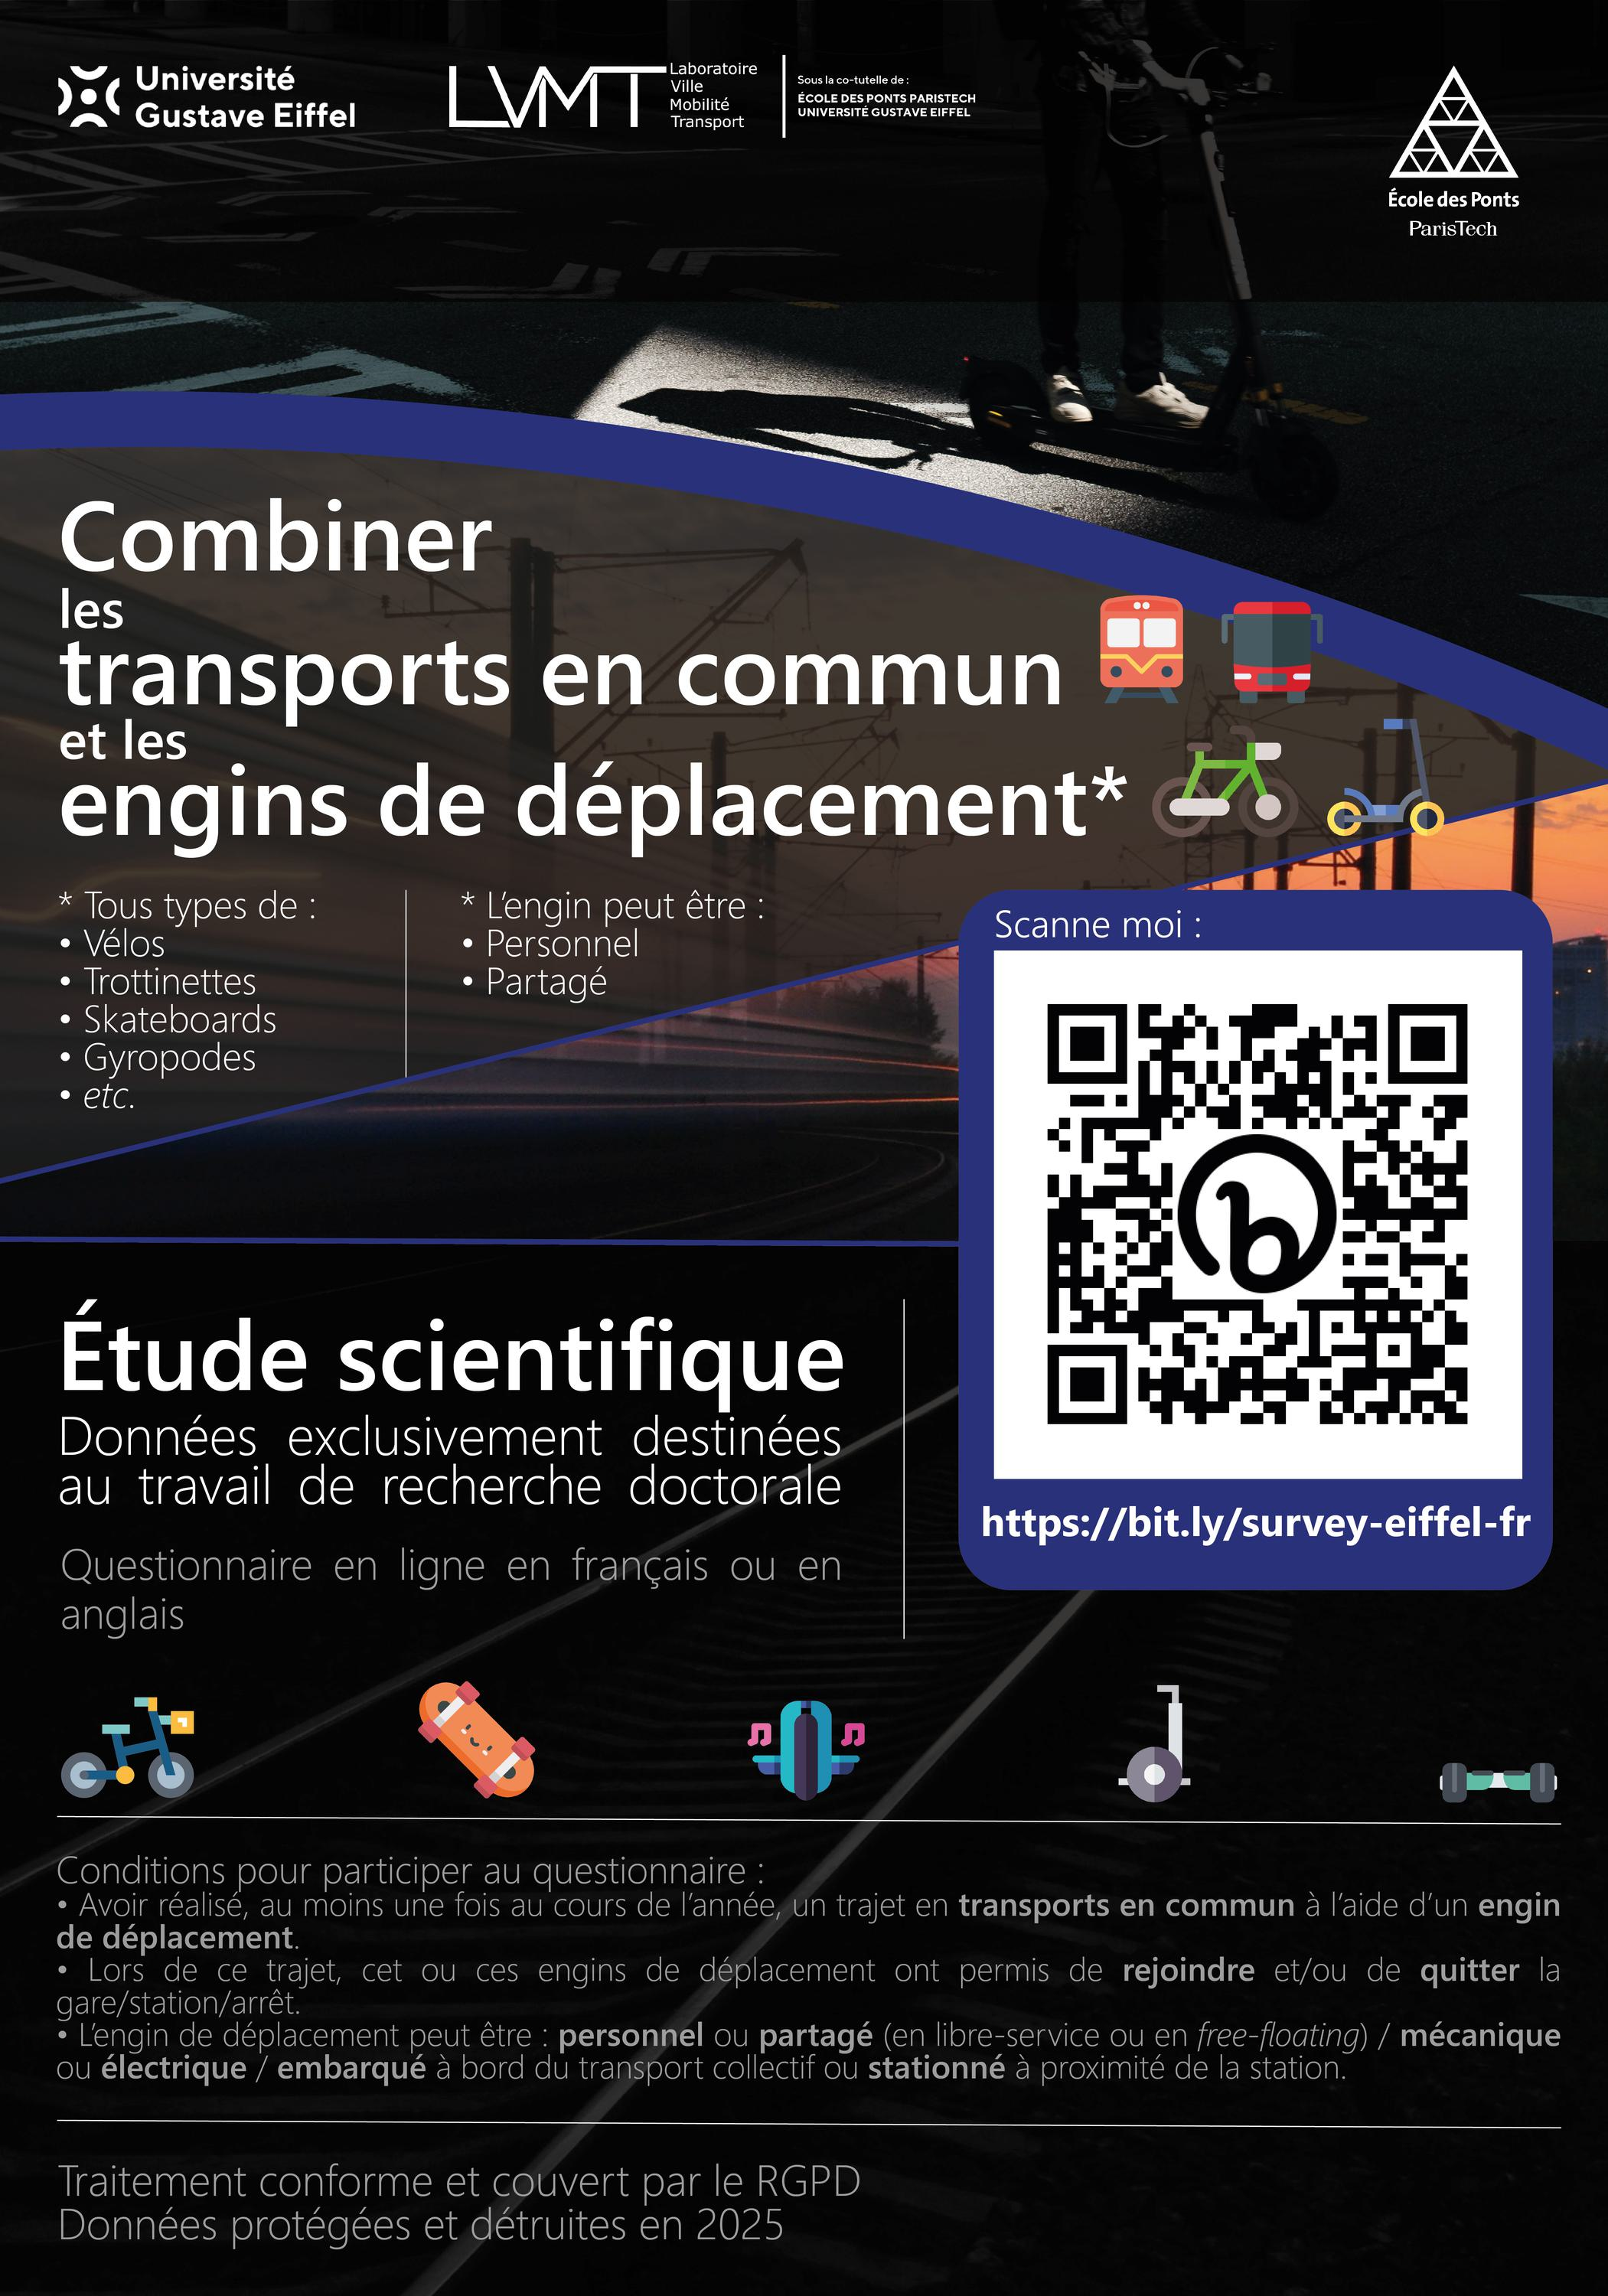
\includegraphics[width=1\columnwidth]{src/Figures/Chap-3/FR_Affiche_Questionnaire.jpg}}
        \vspace{5pt}
        \begin{flushright}\scriptsize{
        Author: \textcolor{blue}{Dylan Moinse (2021)}
        }\end{flushright}
    \end{figure}

    \newpage
    % Questionnaire structure
    \newpage
    \needspace{1\baselineskip} % Reserve space
    \sectionheader{Questionnaire Structure}
\section{Structure of the Survey for Users}
    \label{annexes:structure-questionnaire-usagers}

\textbf{Study on the Combination of Bicycles and Micromobility with Public Transport}

\textsl{You are invited to participate in a research project on the use of public transport in conjunction with bicycles or micromobility options. The survey aims to better understand the mechanisms and challenges of this growing mobility phenomenon from the perspective of mobility and urban planning, with the goal of offering solutions to users.}%%Translated%%

\textsl{To participate in this survey, it is necessary to meet the following condition: having made a trip combining a light mobility mode (bicycle, scooter, \textsl{etc}.) with a public transport mode (train, metro, \textsl{etc}.). By light mobility modes, we refer to bicycles, electric scooters, or other mobility devices, whether personal or shared (bike or scooter in free-floating systems, \textsl{etc}.) and carried aboard public transport or parked or dropped off during the journey.}%%Translated%%

\textsl{This survey takes approximately twenty minutes.}%%Translated%%

\textsl{This study is part of a doctoral thesis at the Laboratoire Ville Mobilité Transport (Gustave Eiffel University and École des Ponts).}%%Translated%%

\textsl{In accordance with the \acrfull{GDPR}, the data collected in this form are anonymized and will be processed exclusively for this research project, namely the collection of social representations and the spatialization of these intermodal trips. The survey takes approximately twenty minutes, and you can stop at any time. It should also be noted that \Marque{LimeSurvey} is a tool promoted by French universities and complies with personal data protection regulations.}%%Translated%%

\textsl{By choosing to participate in this survey:
\begin{customitemize}
    \item You declare that your participation is voluntary and you may, at any time, stop without justification;
    \item You will be able to access the results of the study in its entirety once completed;
    \item The data collected will remain strictly confidential.
\end{customitemize}}%%Translated%%

\textsl{The data usage regulations at Gustave Eiffel University comply with the French Data Protection Act of January 6, 1978, as amended, and with EU Regulation 2016/679 of the European Parliament and Council of April 27, 2016, on the protection of natural persons with regard to the processing of personal data and on the free movement of such data.}%%Translated%%

\textsl{Only the researcher has access to the data, which will be stored for five years. You have the right to contact the \acrfull{DPO} of Gustave Eiffel University or to file a complaint with the \acrfull{CNIL}.}%%Translated%%

\textsl{We sincerely thank you for your participation and interest.}%%Translated%%

    % Questionnaire structure table
% Table T1
%%Translated%%
  \begin{table}[h!]
    \centering
    \renewcommand{\arraystretch}{1.5}
    \resizebox{\columnwidth}{!}{
    \begin{tabular}{p{0.1\columnwidth}p{0.6\columnwidth}p{0.15\columnwidth}p{0.15\columnwidth}}
      % \hline
      \rule{0pt}{15pt} \textcolor{blue}{\textbf{\small{\(T_{1}\)}}} & \textcolor{blue}{\textbf{\small{Question title}}} & \textcolor{blue}{\textbf{\small{Type}}} & \textcolor{blue}{\textbf{\small{Responses}}}\\
      \hline
\multicolumn{4}{l}{\textbf{Consent}}\\
    \small{\textbf{\(Q_{01}^{T_{1}}*\)}} & \small{\textsl{Given the information provided, I freely agree to participate in this research questionnaire.}} & \small{Single choice} & \small{Yes~| No}\\
      \hline
    \end{tabular}}
    \caption*{}
    \vspace{5pt}
        \end{table}

% Table T2
%%Translated%%
  \begin{table}[h!]
    \centering
    \renewcommand{\arraystretch}{1.5}
    \resizebox{\columnwidth}{!}{
    \begin{tabular}{p{0.1\columnwidth}p{0.35\columnwidth}p{0.15\columnwidth}p{0.5\columnwidth}}
      % \hline
      \rule{0pt}{15pt} \textcolor{blue}{\textbf{\small{\(T_{2}\)}}} & \textcolor{blue}{\textbf{\small{Question title}}} & \textcolor{blue}{\textbf{\small{Type}}} & \textcolor{blue}{\textbf{\small{Responses}}}\\
      \hline
\multicolumn{4}{l}{\textbf{Intermodal transport}}\\
    \small{\textbf{\(Q_{01}^{T_{2}}*\)}} & \small{\textsl{Which public transport mode(s) did you use during your last trip that included cycling or a micromobility option?}} & \small{Multiple choice} & \small{\acrshort{HST}~| \acrshort{TERGV}~| \acrshort{TER}~| \acrshort{RER}~| Metro~| Tramway~| Bus~| \textsl{Other(s)}}\\
\hline
    \small{\textbf{\(Q_{02}^{T_{2}}*\)}} & \small{\textsl{What are the departure and arrival (and transfer) stations for this trip made by public transport?}} & \small{Text} & \small{\textsl{Departure station name}~| \textsl{Destination station name}~| \textsl{Transfer station names}}\\
\hline
    \small{\textbf{\(Q_{03}^{T_{2}}*\)}} & \small{\textsl{How did you get from your starting point (your home, if applicable) to the \textcolor{blue}{departure station}?}} & \small{Multiple choice} & \small{Walk~| Bike or micromobility~| Urban public transport~| Car (driver)~| Car (passenger)~| Taxi or \acrshort{RHS}~| Moped or motorcycle~| Car-sharing~| \textsl{Other(s)}}\\
\hline
    \small{\textbf{\(Q_{04}^{T_{2}}*\)}} & \small{\textsl{How would you rate the comfort and quality of this part of the journey from the starting point to the \textcolor{blue}{departure station}?}} & \small{Single choice} & \small{Very positive~| Positive~| Relatively positive~| Relatively negative~| Negative~| Very negative~| I don't know}\\
\hline
    \small{\textbf{\(Q_{05}^{T_{2}}*\)}} & \small{\textsl{How did you get from the \textcolor{blue}{arrival station} to your \textcolor{blue}{destination}?}} & \small{Multiple choice} & \small{Walk~| Light mobility mode~| Urban public transport~| Car (driver)~| Car (passenger)~| Taxi or \acrshort{RHS}~| Moped or motorcycle~| Car-sharing~| \textsl{Other(s)}}\\
\hline
    \small{\textbf{\(Q_{06}^{T_{2}}*\)}} & \small{\textsl{How would you rate the comfort and quality of this part of the journey from the \textcolor{blue}{arrival station} to your destination?}} & \small{Single choice} & \small{Very positive~| Positive~| Relatively positive~| Relatively negative~| Negative~| Very negative~| I don't know}\\
\hline
    \small{\textbf{\(Q_{07}^{T_{2}}*\)}} & \small{\textsl{Which type(s) of bike or micromobility did you use during this combined trip with the \textcolor{blue}{public transport mode(s)}?}} & \small{Multiple choice} & \small{Classic bike~| Folding bike~| Moped~| Skateboard~| Gyroroue or Monowheel~| Hoverboard~| Segway or Gyropod~| \textsl{Other(s)}}\\
\hline
    \small{\textbf{\(Q_{08}^{T_{2}}*\)}} & \small{\textsl{Is your (your) \textcolor{blue}{mode(s) of transport} electric?}} & \small{Single choice} & \small{Yes~| No~| I don't know~| \textsl{Other(s)}}\\
\hline
    \small{\textbf{\(Q_{09}^{T_{2}}*\)}} & \small{\textsl{Do you own your (your) \textcolor{blue}{light individual mobility}?}} & \small{Multiple choice} & \small{Yes, I own it~| No, I use a long-term rental system~| No, I use a shared service~| No, it’s a company vehicle~| No, I borrow it from peers (family, friends, \textsl{etc.})~| \textsl{Other(s)}}\\
\hline
    \small{\textbf{\(Q_{10}^{T_{2}}*\)}} & \small{\textsl{How long have you been using this combination of \textcolor{blue}{light individual mobility} and \textcolor{blue}{public transport mode(s)}?}} & \small{Multiple choice} & \small{For several years~| About a year~| For a few months~| For less than a month~| This was the first time~| I don't know~| \textsl{Other(s)}}\\
\hline
    \small{\textbf{\(Q_{+}^{T_{2}}*\)}} & \small{Open field} & \small{Text} & \small{-}\\
      \hline
    \end{tabular}}
    \caption*{}
    \vspace{5pt}
        \end{table}

% Table T3
%%Translated%%
  \begin{table}[h!]
    \centering
    \renewcommand{\arraystretch}{1.5}
    \resizebox{\columnwidth}{!}{
    \begin{tabular}{p{0.1\columnwidth}p{0.35\columnwidth}p{0.15\columnwidth}p{0.5\columnwidth}}
      % \hline
      \rule{0pt}{15pt} \textcolor{blue}{\textbf{\small{\(T_{3}\)}}} & \textcolor{blue}{\textbf{\small{Question title}}} & \textcolor{blue}{\textbf{\small{Type}}} & \textcolor{blue}{\textbf{\small{Responses}}}\\
      \hline
\multicolumn{4}{l}{\textbf{Geographical landmarks}}\\
    \small{\textbf{\(Q_{01}^{T_{3}}*\)}} & \small{\textsl{What is the location of the starting point (your home, if applicable) of this trip made using \textcolor{blue}{light individual mobility} and \textcolor{blue}{public transport mode(s)}?}} & \small{Text} & \small{Street number~| Street~| Municipality~| Postal code~| Country}\\
\hline
    \small{\textbf{\(Q_{02}^{T_{3}}*\)}} & \small{\textsl{Locate the starting point of this trip on the map.}} & \small{Interactive map} & \small{-}\\
\hline
    \small{\textbf{\(Q_{03}^{T_{3}}*\)}} & \small{\textsl{For this trip from \textcolor{blue}{starting point} to \textcolor{blue}{departure station}, did you take the shortest route possible?}} & \small{Single choice} & \small{Yes~| No~| I don't know~| \textsl{Other(s)}}\\
\hline
    \small{\textbf{\(Q_{04}^{T_{3}}*\)}} & \small{\textsl{What is the location of the destination of this trip made using \textcolor{blue}{light individual mobility} and \textcolor{blue}{public transport mode(s)}?}} & \small{Text} & \small{Street number~| Street~| Municipality~| Postal code~| Country}\\
\hline
    \small{\textbf{\(Q_{05}^{T_{3}}*\)}} & \small{\textsl{Locate the destination of this trip on the map.}} & \small{Interactive map} & \small{-}\\
\hline
    \small{\textbf{\(Q_{06}^{T_{3}}*\)}} & \small{\textsl{For this trip from \textcolor{blue}{arrival station} to \textcolor{blue}{destination}, did you take the shortest route possible?}} & \small{Single choice} & \small{Yes~| No~| I don't know~| \textsl{Other(s)}}\\
\hline
    \small{\(C_{01}^{T_{3}}*\)} & \small{\textsl{You answered that you did not take the shortest route. What was the reason(s) for taking a detour?}} & \small{Multiple choice} & \small{Traveling on a road with less traffic~| Traveling on a road with a lower speed limit~| Traveling on a cycling or pedestrian infrastructure~| Avoiding cobblestones~| Avoiding degraded roads (potholes, poor surface quality, \textsl{etc.})~| Avoiding a dangerous intersection (roundabout, junction, \textsl{etc.})~| Avoiding a sloped terrain (hill)~| For secondary activities (shopping, escorting, social interaction, walking, \textsl{etc.})~| \textsl{Other(s)}}\\
\hline
    \small{\textbf{\(Q_{07}^{T_{3}}*\)}} & \small{\textsl{Do you sometimes make intermediate stops (pauses) during this intermodal trip?}} & \small{Single choice} & \small{Constantly~| Regularly~| Occasionally~| Rarely~| Never~| I don't know}\\
\hline
    \small{\(C_{02}^{T_{3}}*\)} & \small{\textsl{You answered that you made intermediate stops during the trip. Could you specify the type of secondary activity that occurred during the trip?}} & \small{Multiple choice} & \small{Professional or educational reasons~| Shopping~| Escorting~| Leisure~| Meeting peers (family, friends, \textsl{etc.})~| Administrative or medical reasons~| Walking~| \textsl{Other(s)}}\\
\hline
    \small{\textbf{\(Q_{+}^{T_{3}}*\)}} & \small{Open field} & \small{Text} & \small{-}\\
      \hline
    \end{tabular}}
    \caption*{}
    \vspace{5pt}
        \end{table}

% Table T4
%%Translated%%
  \begin{table}[h!]
    \centering
    \renewcommand{\arraystretch}{1.5}
    \resizebox{\columnwidth}{!}{
    \begin{tabular}{p{0.1\columnwidth}p{0.35\columnwidth}p{0.15\columnwidth}p{0.5\columnwidth}}
      % \hline
      \rule{0pt}{15pt} \textcolor{blue}{\textbf{\small{\(T_{4}\)}}} & \textcolor{blue}{\textbf{\small{Question title}}} & \textcolor{blue}{\textbf{\small{Type}}} & \textcolor{blue}{\textbf{\small{Responses}}}\\
      \hline
\multicolumn{4}{l}{\textbf{Parking and boarding practices}}\\
    \small{\textbf{\(Q_{01}^{T_{4}}*\)}} & \small{\textsl{Did you board your \textcolor{blue}{light individual mobility} on the \textcolor{blue}{public transport mode(s)}?}} & \small{Single choice} & \small{Yes~| No~| Not throughout the public transport journey~| I don't know~| \textsl{Other(s)}}\\
\hline
    \small{\(C_{01}^{T_{4}}*\)} & \small{\textsl{You answered that you boarded your \textcolor{blue}{light individual mobility}. What are the reasons for this intermodal practice?}} & \small{Multiple choice} & \small{No parking near the stations~| Insecure parking~| To be able to use it upon arriving at \textcolor{blue}{arrival station}~| I don't know~| \textsl{Other(s)}}\\
\hline
    \small{\(C_{02}^{T_{4}}*\)} & \small{\textsl{You answered that you boarded your \textcolor{blue}{light individual mobility}. Do you consider boarding the vehicle generally simple?}} & \small{Single choice} & \small{Yes~| No~| I don't know~| \textsl{Other(s)}}\\
\hline
    \small{\(C_{03}^{T_{4}}*\)} & \small{\textsl{You answered that boarding your \textcolor{blue}{light individual mobility} is complex. What are the major obstacles you face when boarding your vehicle(s)?}} & \small{Multiple choice} & \small{No appropriate or dedicated space for this vehicle(s)~| Not enough space in this dedicated space~| Weight of the vehicle(s)~| Physical barriers (gates, stairs, \textsl{etc.})~| I don't know~| \textsl{Other(s)}}\\
\hline
    \small{\(C_{04}^{T_{4}}*\)} & \small{\textsl{You answered that you partially boarded your \textcolor{blue}{light individual mobility}. In which public transport mode(s) did you board it?}} & \small{Multiple choice} & \small{\acrshort{HST}~| \acrshort{TERGV}~| \acrshort{TER}~| \acrshort{RER}~| Metro~| Tramway~| Bus~| I don't know~| \textsl{Other(s)}}\\
\hline
    \small{\(C_{05}^{T_{4}}*\)} & \small{\textsl{You answered that you did not board (fully or partially) your \textcolor{blue}{light individual mobility}. Where did you park it?}} & \small{Multiple choice} & \small{In a bike station or bike locker near the \textcolor{blue}{departure station}~| Locked to a bike rack~| In a public protected parking area~| In a private protected parking area~| I don't know~| \textsl{Other(s)}}\\
\hline
    \small{\(C_{06}^{T_{4}}*\)} & \small{\textsl{You answered that you boarded your \textcolor{blue}{light individual mobility}. If a protected, free parking space designated for your vehicle(s) was provided at your public transport stations, would you use it?}} & \small{Single choice} & \small{Yes~| No~| I don't know~| \textsl{Other(s)}}\\
\hline
    \small{\textbf{\(Q_{+}^{T_{4}}\)}} & \small{Open field} & \small{Text} & \small{-}\\
      \hline
    \end{tabular}}
    \caption*{}
    \vspace{5pt}
        \end{table}

% Table T5
%%Translated%%
  \begin{table}[h!]
    \centering
    \renewcommand{\arraystretch}{1.5}
    \resizebox{\columnwidth}{!}{
    \begin{tabular}{p{0.1\columnwidth}p{0.35\columnwidth}p{0.15\columnwidth}p{0.5\columnwidth}}
      % \hline
      \rule{0pt}{15pt} \textcolor{blue}{\textbf{\small{\(T_{5}\)}}} & \textcolor{blue}{\textbf{\small{Question title}}} & \textcolor{blue}{\textbf{\small{Type}}} & \textcolor{blue}{\textbf{\small{Responses}}}\\
      \hline
\multicolumn{4}{l}{\textbf{Characteristics of the intermodal trip}}\\
    \small{\textbf{\(Q_{01}^{T_{5}}*\)}} & \small{\textsl{How often do you make this trip using \textcolor{blue}{light individual mobility} and \textcolor{blue}{public transport mode(s)}?}} & \small{Single choice} & \small{At least five times a week~| Several times a week~| Once a week~| Several times a month~| Once a month~| Several times a year~| This was the first time~| I don't know~| \textsl{Other(s)}}\\
\hline
    \small{\textbf{\(Q_{02}^{T_{5}}*\)}} & \small{\textsl{For what reason(s) did you make this trip using \textcolor{blue}{light individual mobility} and \textcolor{blue}{public transport mode(s)}?}} & \small{Multiple choice} & \small{Home - Work~| Home - Studies~| Shopping~| Leisure or vacation~| Visits or walks~| Administrative or medical~| I don't know~| \textsl{Other(s)}}\\
\hline
    \small{\textbf{\(Q_{03}^{T_{5}}*\)}} & \small{\textsl{Rank the top five reasons (in descending order, with 1 being the most important) why you adopted this form of travel.}} & \small{Interactive ranking} & \small{Public and private subsidies~| Word of mouth~| Fuel cost~| Comfort~| Curiosity~| Moving~| Too long distances on foot~| Eco-friendly~| Flexibility~| Freedom of movement~| Fun~| Mimicry~| No alternative~| Door-to-door~| Getting fresh air~| Cycling network~| I don't know~| Other}\\
\hline
    \small{\(C_{01}^{T_{5}}*\)} & \small{\textsl{You answered "Other" (in position 1, 2, 3, 4, or 5). Please specify the other reason that influenced your ranking.}} & \small{Text} & \small{-}\\
\hline
    \small{\textbf{\(Q_{04}^{T_{5}}*\)}} & \small{\textsl{If you couldn't have used your (your) \textcolor{blue}{light individual mobility}, how would you have reached the \textcolor{blue}{departure station}?}} & \small{Multiple choice} & \small{I would have reached \textcolor{blue}{departure station} in another way~| I would have reached another departure station in another way~| I wouldn't have taken public transport~| I wouldn't have made the trip at all~| I don't know~| \textsl{Other(s)}}\\
\hline
   \small{\(C_{02}^{T_{5}}*\)} & \small{\textsl{You answered that you would have reached \textcolor{blue}{departure station} in another way. With what mode(s) of transport?}} & \small{Multiple choice} & \small{Walk~| Urban public transport~| Car (driver)~| Car (passenger)~| Taxi or \acrshort{RHS}~| Moped or motorcycle~| Car-sharing~| I don't know~| \textsl{Other(s)}}\\
\hline
   \small{\(C_{03}^{T_{5}}*\)} & \small{\textsl{You answered that you wouldn't have taken public transport. What solution(s) would you have used to replace the entire trip?}} & \small{Multiple choice} & \small{Walk~| Urban public transport~| Car (driver)~| Car (passenger)~| Taxi or \acrshort{RHS}~| Moped or motorcycle~| Car-sharing~| I don't know~| \textsl{Other(s)}}\\
\hline
   \small{\textbf{\(Q_{05}^{T_{5}}*\)}} & \small{\textsl{If you couldn't have used your (your) \textcolor{blue}{light individual mobility}, how would you have traveled from \textcolor{blue}{arrival station} to \textcolor{blue}{destination}?}} & \small{Multiple choice} & \small{I would have left \textcolor{blue}{arrival station} in another way~| I would have left another arrival station in another way~| I wouldn't have taken public transport~| I wouldn't have made the trip at all~| I don't know~| \textsl{Other(s)}}\\
\hline
   \small{\(C_{04}^{T_{5}}*\)} & \small{\textsl{You answered that you would have traveled from \textcolor{blue}{arrival station} to \textcolor{blue}{destination} in another way. With what mode(s) of transport?}} & \small{Multiple choice} & \small{Walk~| Urban public transport~| Car (driver)~| Car (passenger)~| Taxi or \acrshort{RHS}~| Moped or motorcycle~| Car-sharing~| I don't know~| \textsl{Other(s)}}\\
\hline
   \small{\(C_{05}^{T_{5}}*\)} & \small{\textsl{You answered that you wouldn't have taken public transport. What solution(s) would you have used to replace the entire trip?}} & \small{Multiple choice} & \small{Walk~| Urban public transport~| Car (driver)~| Car (passenger)~| Taxi or \acrshort{RHS}~| Moped or motorcycle~| Car-sharing~| I don't know~| \textsl{Other(s)}}\\
\hline
   \small{\textbf{\(Q_{06}^{T_{5}}*\)}} & \small{\textsl{In general, what solution(s) would you propose to improve your trip?}} & \small{Text} & \small{-}\\
   \small{\textbf{\(Q_{+}^{T_{5}}*\)}} & \small{Open field} & \small{Text} & \small{-}\\
      \hline
    \end{tabular}}
    \caption*{}
    \vspace{5pt}
        \end{table}

% Table T6
%%Translated%%
  \begin{table}[h!]
    \centering
    \renewcommand{\arraystretch}{1.5}
    \resizebox{\columnwidth}{!}{
    \begin{tabular}{p{0.1\columnwidth}p{0.35\columnwidth}p{0.15\columnwidth}p{0.5\columnwidth}}
      % \hline
      \rule{0pt}{15pt} \textcolor{blue}{\textbf{\small{\(T_{6}\)}}} & \textcolor{blue}{\textbf{\small{Question title}}} & \textcolor{blue}{\textbf{\small{Type}}} & \textcolor{blue}{\textbf{\small{Responses}}}\\
      \hline
\multicolumn{4}{l}{\textbf{Mobility habits}}\\
   \small{\textbf{\(Q_{01}^{T_{6}}*\)}} & \small{\textsl{Check the boxes corresponding to the frequency of use of these modes of transport (Walking~| Public transport~| Personal bike~| \acrshort{PeS}~| \acrshort{PBS}~| \acrshort{DESS}~| Car (driver)~| Car (passenger)~| Taxi or \acrshort{RHS}~| Moped or motorcycle~| Car-sharing).}} & \small{Interactive table} & \small{Never~| Rarely~| Occasionally~| Often~| Daily~| I don't know}\\
\hline
   \small{\textbf{\(Q_{02}^{T_{6}}*\)}} & \small{\textsl{Do you currently have a public transport subscription?}} & \small{Single choice} & \small{Yes~| No~| I don't know~| \textsl{Other(s)}}\\
\hline
   \small{\textbf{\(Q_{03}^{T_{6}}*\)}} & \small{\textsl{Do you currently have a \acrshort{PBS} or \acrshort{DESS} subscription?}} & \small{Single choice} & \small{Yes~| No~| I don't know~| \textsl{Other(s)}}\\
\hline
   \small{\textbf{\(Q_{04}^{T_{6}}*\)}} & \small{\textsl{Do you currently have a car-sharing or Moped rental subscription?}} & \small{Single choice} & \small{Yes~| No~| I don't know~| \textsl{Other(s)}}\\
\hline
   \small{\textbf{\(Q_{05}^{T_{6}}*\)}} & \small{\textsl{Do you currently have a driver's license?}} & \small{Single choice} & \small{Yes~| No~| I don't know~| \textsl{Other(s)}}\\
\hline
   \small{\textbf{\(Q_{06}^{T_{6}}*\)}} & \small{\textsl{Is your household motorized?}} & \small{Single choice} & \small{Yes~| No~| I don't know~| \textsl{Other(s)}}\\
\hline
   \small{\(C_{01}^{T_{6}}*\)} & \small{\textsl{You answered that you are motorized. How many private cars does your household own?}} & \small{Numeric} & \small{-}\\
\hline
   \small{\textbf{\(Q_{07}^{T_{6}}*\)}} & \small{\textsl{Do you own one or more bicycles?}} & \small{Single choice} & \small{Yes~| No~| I don't know~| \textsl{Other(s)}}\\
\hline
   \small{\textbf{\(Q_{08}^{T_{6}}*\)}} & \small{\textsl{Do you use these modes of transport more or less often since you started using \textcolor{blue}{light individual mobility} and \textcolor{blue}{public transport mode(s)} (Walking~| Public transport~| Personal bike~| \acrshort{PeS}~| \acrshort{PBS}~| \acrshort{DESS}~| Car (driver)~| Car (passenger)~| Taxi or \acrshort{RHS}~| Moped or motorcycle~| Car-sharing)?}} & \small{Interactive table} & \small{Much less often~| Less often~| At the same frequency~| More often~| Much more often~| I don't know}\\
\hline
   \small{\textbf{\(Q_{09}^{T_{6}}*\)}} & \small{\textsl{In your opinion, are the following elements important for achieving an ideal territory (High density~| Sprawling housing~| Mixed-use~| Pedestrian network~| Cycling network~| Public transport network~| Car restrictions up to one kilometer around stations~| Car restrictions up to three kilometers around stations)?}} & \small{Interactive table} & \small{Favorable~| Acceptable~| Unacceptable~| Hostile~| I don't know}\\
\hline
   \small{\textbf{\(Q_{10}^{T_{6}}*\)}} & \small{\textsl{In your opinion, what are the most important criteria for choosing a place to live?}} & \small{Multiple choice} & \small{Accessible within ten minutes on foot from a station~| Accessible within twenty minutes on foot from a station~| Accessible within ten minutes by bike or micromobility from a station~| Green spaces nearby~| Old collective housing~| New collective housing~| Individual housing in a dense area~| Individual suburban housing~| Commercial offerings nearby~| Cultural offerings nearby~| Parking space(s) for cars~| Parking space(s) for bikes~| Affordable purchase or rental price~| Housing area size}\\
\hline
    \small{\textbf{\(Q_{+}^{T_{6}}*\)}} & \small{Open field} & \small{Text} & \small{-}\\
      \hline
    \end{tabular}}
    \caption*{}
    \vspace{5pt}
        \end{table}

% Table T7
%%Translated%%
  \begin{table}[h!]
    \centering
    \renewcommand{\arraystretch}{1.5}
    \resizebox{\columnwidth}{!}{
    \begin{tabular}{p{0.1\columnwidth}p{0.35\columnwidth}p{0.15\columnwidth}p{0.5\columnwidth}}
      % \hline
      \rule{0pt}{15pt} \textcolor{blue}{\textbf{\small{\(T_{7}\)}}} & \textcolor{blue}{\textbf{\small{Question title}}} & \textcolor{blue}{\textbf{\small{Type}}} & \textcolor{blue}{\textbf{\small{Responses}}}\\
      \hline
\multicolumn{4}{l}{\textbf{Socio-demographic profile}}\\
   \small{\textbf{\(Q_{01}^{T_{7}}\)}} & \small{\textsl{Which gender identity do you identify with most?}} & \small{Multiple choice} & \small{Female~| Male~| I prefer not to say~| \textsl{Other(s)}}\\
\hline
   \small{\textbf{\(Q_{02}^{T_{7}}\)}} & \small{\textsl{What is your age?}} & \small{Numeric} & \small{-}\\
\hline
   \small{\textbf{\(Q_{03}^{T_{7}}\)}} & \small{\textsl{What is your household composition?}} & \small{Single choice} & \small{Single~| Couple without children~| Couple with one child~| Couple with multiple children~| Single with one or more child(ren)~| In shared accommodation~| \textsl{Other(s)}}\\
\hline
   \small{\textbf{\(Q_{04}^{T_{7}}\)}} & \small{\textsl{What is your current status?}} & \small{Single choice} & \small{Full-time employed~| Part-time employed~| Job seeker~| Student in training~| Student with a job~| At home~| Retired~| \textsl{Other(s)}}\\
\hline
   \small{\textbf{\(Q_{05}^{T_{7}}\)}} & \small{\textsl{Which profession and socio-professional category do you belong to or have belonged to most recently?}} & \small{Single choice} & \small{Farmers~| Artisans, traders, and business owners~| Managers and higher intellectual professions~| Intermediate professions~| Employees~| Workers~| \textsl{Other(s)}}\\
\hline
   \small{\textbf{\(Q_{06}^{T_{7}}\)}} & \small{\textsl{What is the highest degree you have obtained?}} & \small{Single choice} & \small{No diploma~| BEP, CAP or equivalent~| High school diploma~| Bac+2 (BTS, DUT, \textsl{etc.})~| Bac+3 (Bachelor's degree)~| Bac+5 (Master's, Engineer, \textsl{etc.})~| Bac+6 or higher (Mastère, PhD, HDR, \textsl{etc.})~| I prefer not to answer~| \textsl{Other(s)}}\\
\hline
   \small{\textbf{\(Q_{07}^{T_{7}}\)}} & \small{\textsl{How much do you estimate your household's monthly disposable income to be?}} & \small{Numeric} & \small{-}\\
\hline
    \small{\textbf{\(Q_{+}^{T_{7}}\)}} & \small{Open field} & \small{Text} & \small{-}\\
      \hline
    \end{tabular}}
    \caption*{}
    \vspace{5pt}
        \end{table}

% Table T8
%%Translated%%
  \begin{table}[h!]
    \centering
    \renewcommand{\arraystretch}{1.5}
    \resizebox{\columnwidth}{!}{
    \begin{tabular}{p{0.1\columnwidth}p{0.35\columnwidth}p{0.15\columnwidth}p{0.5\columnwidth}}
      % \hline
      \rule{0pt}{15pt} \textcolor{blue}{\textbf{\small{\(T_{8}\)}}} & \textcolor{blue}{\textbf{\small{Question title}}} & \textcolor{blue}{\textbf{\small{Type}}} & \textcolor{blue}{\textbf{\small{Responses}}}\\
      \hline
\multicolumn{4}{l}{\textbf{End of the questionnaire}}\\
   \small{\textbf{\(Q_{01}^{T_{8}}\)*}} & \small{\textsl{If you would like to participate, we are looking for volunteers to conduct an interview on the ground, following you throughout your trip using \textcolor{blue}{light individual mobility} and \textcolor{blue}{public transport mode(s).}}} & \small{Single choice} & \small{Yes~| No}\\
\hline
   \small{\(C_{01}^{T_{8}}\)} & \small{\textsl{You answered that you are interested in participating in an interview. Please feel free to share your email address or phone number so that we can contact you. To maintain the anonymity of your response, please send it to us by email at \textcolor{blue}{dylan.moinse@univ-eiffel.fr}.}} & \small{Text} & \small{-}\\
\hline
   \small{\textbf{\(Q_{02}^{T_{8}}\)}} & \small{\textsl{If you wish to add additional information or make comments, you can freely express yourself here. You can also email us at \textcolor{blue}{dylan.moinse@univ-eiffel.fr} if you would like to receive the survey results.}} & \small{Text} & \small{-}\\
      \hline
    \end{tabular}}
    \caption*{}
    \vspace{5pt}
        \begin{flushleft}\scriptsize
        Note: \(T\) refers to a general theme, \(Q\) refers to a question, and \(C\) refers to a conditional question.
        \end{flushleft}
        \begin{flushright}\scriptsize
        Author: \textcolor{blue}{Dylan Moinse (2021)}
        \end{flushright}
        \end{table}%%Translated%%